\documentclass{report}

\usepackage{hyperref}

\usepackage{epstopdf}
\usepackage{amsmath}
\usepackage{amssymb}
\usepackage{subfig}
%\usepackage{multirow}
\usepackage[utf8]{inputenc}
\usepackage[T1]{fontenc}
\usepackage{standalone}
\usepackage{tikz}
\usepackage{tabularx}
\usepackage{float}
\usepackage[section]{placeins}
\usepackage{sverb}
\usepackage{import}
\usepackage{verbatim}
\usepackage{listings}
\usepackage{xcolor}

\graphicspath{{img/}}
\DeclareGraphicsExtensions{.pdf,.png,.jpg,.svg} %For pdflatex



\begin{document}

\begin{titlepage}
    \begin{center}
        
\includegraphics[width=.50\linewidth]{polsl.png}\\
        \Huge
        \textbf{Przetwarzanie Obrazów Cyfrowych}
        \\ \vspace{1.5cm}
        \Large
        \textbf{Raport z ćwiczenia 3}        
    \end{center}
    \vspace{3.0cm}
    \Large
    Raport opracował:\\
    Dawid Kania\\
    Grupa 6 Semestr 6\\ \\ 
    Data wykonania ćwiczenia: 28.04.2022\\
\end{titlepage}


\section*{
    Obliczanie liczby barw w obrazie
}


\newcommand{\ww}{0.45} %zmienna używana jako parametr opisujące szerokość obrazu zdefiniowana poraz pierwszy w dokumencie
\begin{figure}[H]
    \captionsetup[subfloat]{justification=raggedright,singlelinecheck=false, position=bottom,labelformat=empty} %
    \subfloat[POClab = 54450 \\ RGB = 54450  \\ HSV = 54450 \\ YCbCr = 54450 \\ czas =  1.6995 s ]{\includegraphics[width=\ww\linewidth]{../obrazy/05\_512x512.png }} \hfill%	
    \subfloat[POClab = 230651 \\ RGB = 230651  \\ HSV = 230651 \\ YCbCr = 230651 \\ czas =  26.3035 s ]{\includegraphics[width=\ww\linewidth]{../obrazy/baboon\_512x512.png  }} \hfill% wypełnenie
    \caption{obliczanie liczby barw w obrazie} 
    \label{fig:porownanie1} %label który można wykorzystać w tekście za pomocą polecenia \ref{fig:porownanie1}
\end{figure}


\begin{figure}[H]
    \captionsetup[subfloat]{justification=raggedright,singlelinecheck=false, position=bottom,labelformat=empty} %
    \subfloat[POClab = 148702 \\ RGB = 148702  \\ HSV = 148702 \\ YCbCr = 148702 \\ czas =  9.3294 s ]{\includegraphics[width=\ww\linewidth]{../obrazy/lena\_512x512.png     }} \hfill%	
    \subfloat[POClab = 111344 \\ RGB = 111344  \\ HSV = 111344 \\ YCbCr = 111344 \\ czas =  4.9705 s ]{\includegraphics[width=\ww\linewidth]{../obrazy/peppers3\_512x512.png }} \hfill% wypełnenie
    \caption{obliczanie liczby barw w obrazie} 
    \label{fig:porownanie1} %label który można wykorzystać w tekście za pomocą polecenia \ref{fig:porownanie1}
\end{figure}



\section*{
    Kwantyzacja obrazów
}

\subsection*{
    Kwantyzacja RGB
}

\renewcommand{\ww}{0.19} 
\begin{figure}[H]
    \captionsetup[subfloat]{justification=raggedright,singlelinecheck=false, position=bottom,labelformat=empty} %
    \subfloat[Oryginał \\ Liczba barw = 230651]{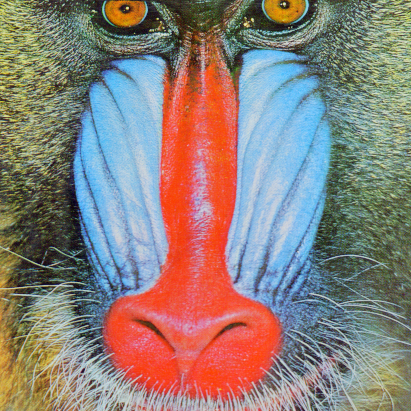
\includegraphics[width=\ww\linewidth]{../zad2/rgb1/I1_ori.png }} \hfill%	
    \subfloat[Kwant. 2x2x2 \\ Liczba barw = 8 \\ PSNR = 17.4004]{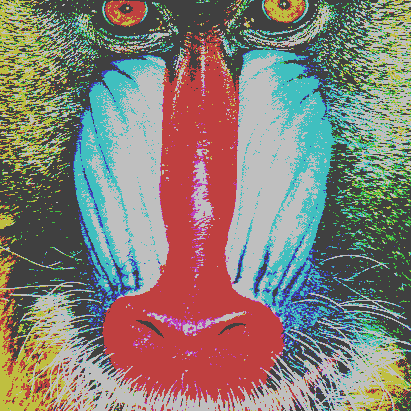
\includegraphics[width=\ww\linewidth]{../zad2/rgb1/I1_222.png }} \hfill%	
    \subfloat[Kwant. 4x4x4 \\ Liczba barw = 50 \\ PSNR = 22.7052]{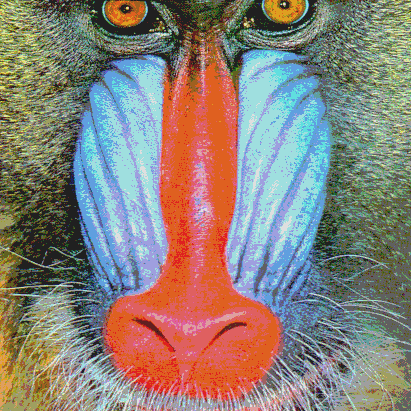
\includegraphics[width=\ww\linewidth]{../zad2/rgb1/I1_444.png }} \hfill% wypełnenie
    \subfloat[Kwant. 4x6x4 \\ Liczba barw = 68 \\ PSNR = 23.8425]{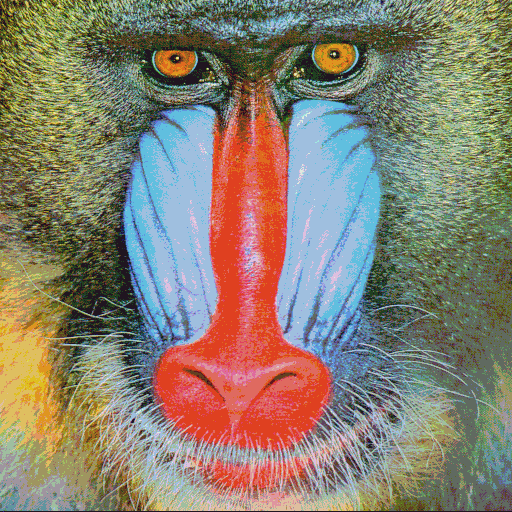
\includegraphics[width=\ww\linewidth]{../zad2/rgb1/I1_464.png }} \hfill%	
    \subfloat[Kwant. 8x8x4 \\ Liczba barw = 148 \\ PSNR = 26.0180]{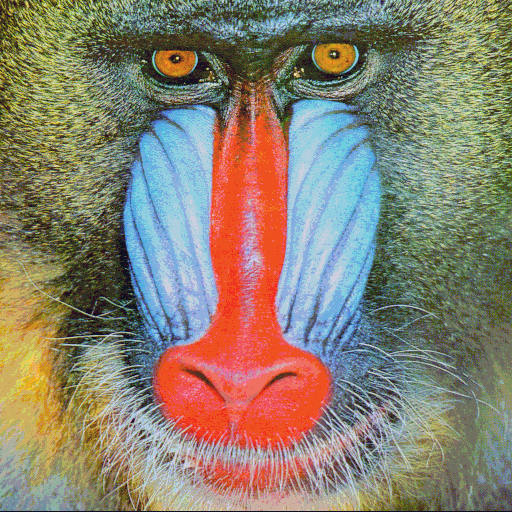
\includegraphics[width=\ww\linewidth]{../zad2/rgb1/I1_884.png }} \hfill% wypełnenie
    \caption{skwantyzowane obrazy RGB} 
    \label{fig:porownanie1} %label który można wykorzystać w tekście za pomocą polecenia \ref{fig:porownanie1}
\end{figure}

\renewcommand{\ww}{0.19} 
\begin{figure}[H]
    \captionsetup[subfloat]{justification=raggedright,singlelinecheck=false, position=bottom,labelformat=empty} %
    \subfloat[Oryginał \\ Liczba barw = 148702]{\includegraphics[width=\ww\linewidth]{../zad2/rgb2/I1_ori.png }} \hfill%	
    \subfloat[Kwant. 2x2x2 \\ Liczba barw = 6 \\ PSNR = 17.2712]{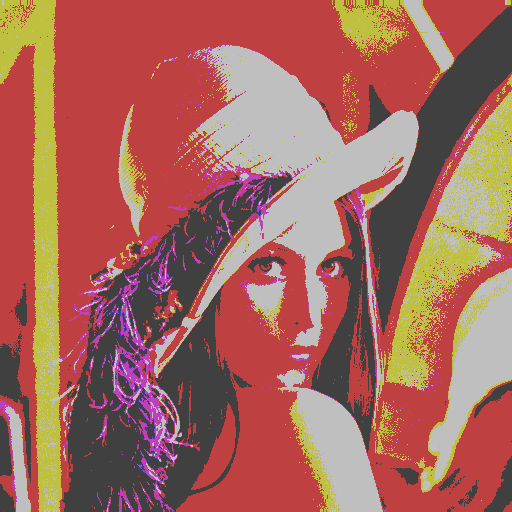
\includegraphics[width=\ww\linewidth]{../zad2/rgb2/I1_222.png }} \hfill%	
    \subfloat[Kwant. 4x4x4 \\ Liczba barw = 28 \\ PSNR = 22.9811]{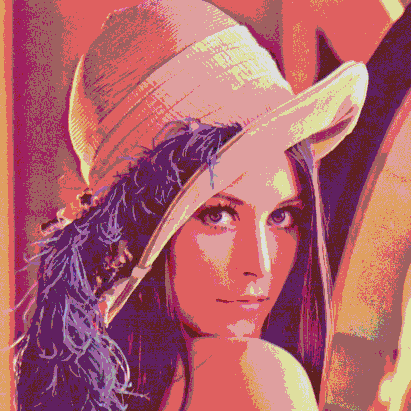
\includegraphics[width=\ww\linewidth]{../zad2/rgb2/I1_444.png }} \hfill% wypełnenie
    \subfloat[Kwant. 4x6x4 \\ Liczba barw = 41 \\ PSNR = 24.0248]{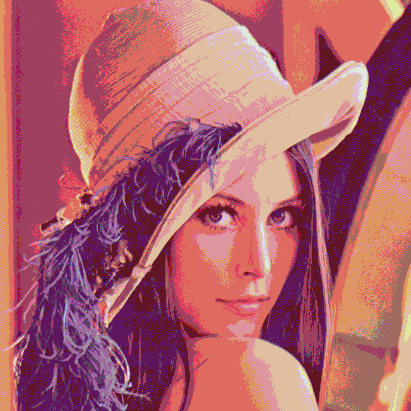
\includegraphics[width=\ww\linewidth]{../zad2/rgb2/I1_464.png }} \hfill%	
    \subfloat[Kwant. 8x8x4 \\ Liczba barw = 74 \\ PSNR = 25.4516]{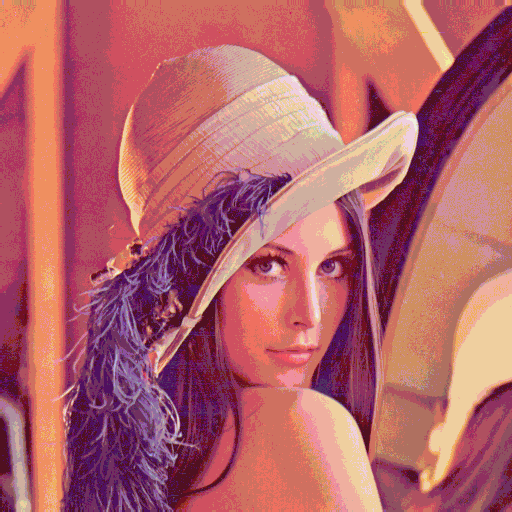
\includegraphics[width=\ww\linewidth]{../zad2/rgb2/I1_884.png }} \hfill% wypełnenie
    \caption{skwantyzowane obrazy RGB} 
    \label{fig:porownanie1} %label który można wykorzystać w tekście za pomocą polecenia \ref{fig:porownanie1}
\end{figure}

\renewcommand{\ww}{0.19} 
\begin{figure}[H]
    \captionsetup[subfloat]{justification=raggedright,singlelinecheck=false, position=bottom,labelformat=empty} %
    \subfloat[Oryginał \\ Liczba barw = 111344]{\includegraphics[width=\ww\linewidth]{../zad2/rgb3/I1_ori.png }} \hfill%	
    \subfloat[Kwant. 2x2x2 \\ Liczba barw = 7 \\ PSNR = 17.4608]{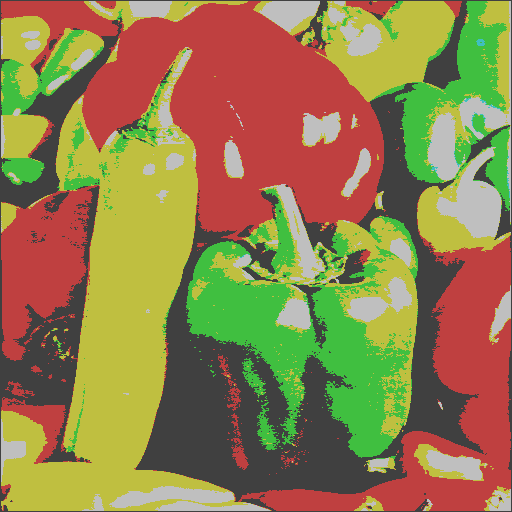
\includegraphics[width=\ww\linewidth]{../zad2/rgb3/I1_222.png }} \hfill%	
    \subfloat[Kwant. 4x4x4 \\ Liczba barw = 33 \\ PSNR = 22.4221]{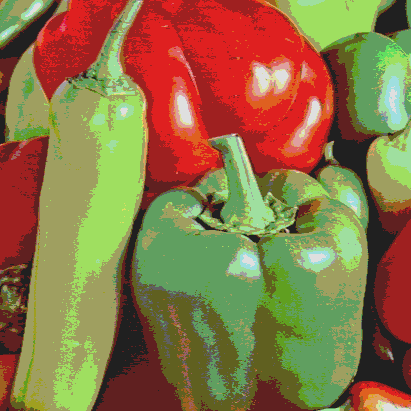
\includegraphics[width=\ww\linewidth]{../zad2/rgb3/I1_444.png }} \hfill% wypełnenie
    \subfloat[Kwant. 4x6x4 \\ Liczba barw = 45 \\ PSNR = 23.3479]{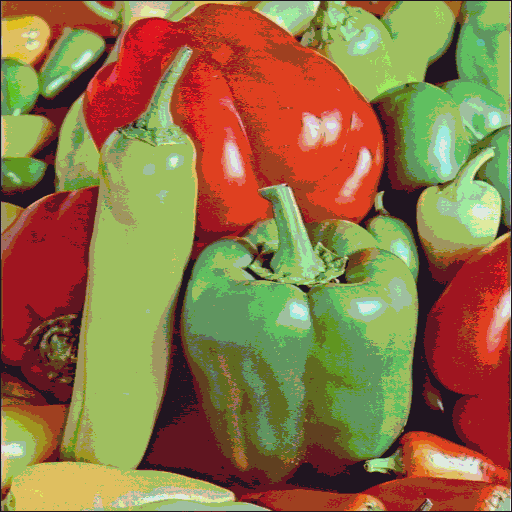
\includegraphics[width=\ww\linewidth]{../zad2/rgb3/I1_464.png }} \hfill%	
    \subfloat[Kwant. 8x8x4 \\ Liczba barw = 93 \\ PSNR = 25.9188]{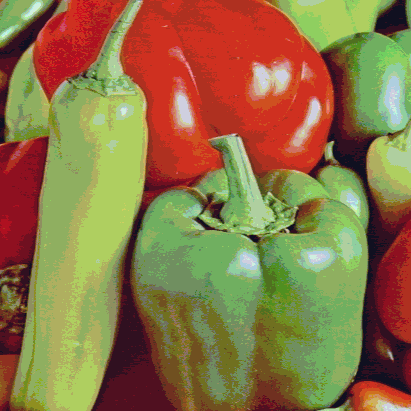
\includegraphics[width=\ww\linewidth]{../zad2/rgb3/I1_884.png }} \hfill% wypełnenie
    \caption{skwantyzowane obrazy RGB} 
    \label{fig:porownanie1} %label który można wykorzystać w tekście za pomocą polecenia \ref{fig:porownanie1}
\end{figure}

\renewcommand{\ww}{0.19} 
\begin{figure}[H]
    \captionsetup[subfloat]{justification=raggedright,singlelinecheck=false, position=bottom,labelformat=empty} %
    \subfloat[Oryginał \\ Liczba barw = 188833]{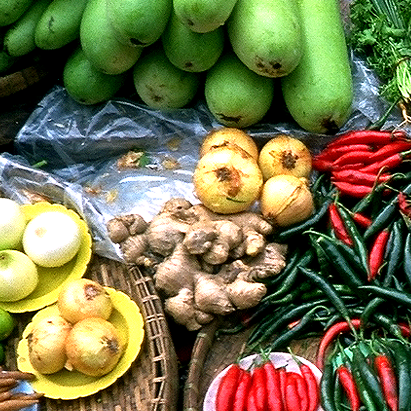
\includegraphics[width=\ww\linewidth]{../zad2/rgb4/I1_ori.png }} \hfill%	
    \subfloat[Kwant. 2x2x2 \\ Liczba barw = 8 \\ PSNR = 15.3367]{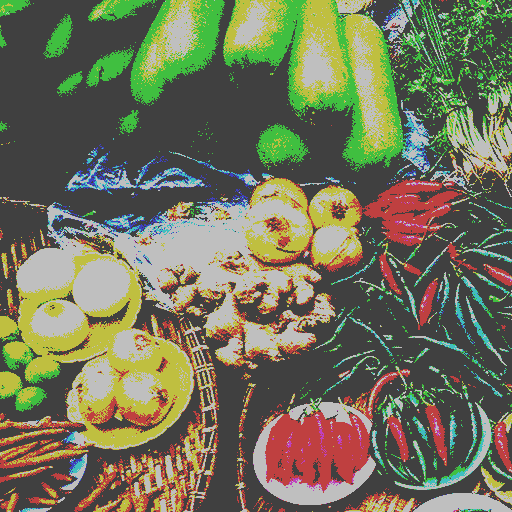
\includegraphics[width=\ww\linewidth]{../zad2/rgb4/I1_222.png }} \hfill%	
    \subfloat[Kwant. 4x4x4 \\ Liczba barw = 53 \\ PSNR = 21.3802]{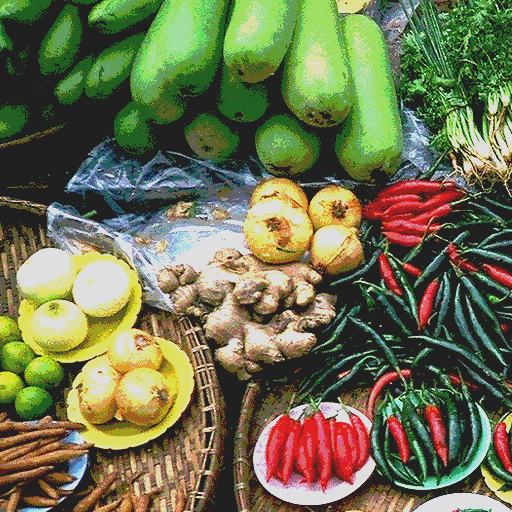
\includegraphics[width=\ww\linewidth]{../zad2/rgb4/I1_444.png }} \hfill% wypełnenie
    \subfloat[Kwant. 4x6x4 \\ Liczba barw = 76 \\ PSNR = 22.1796]{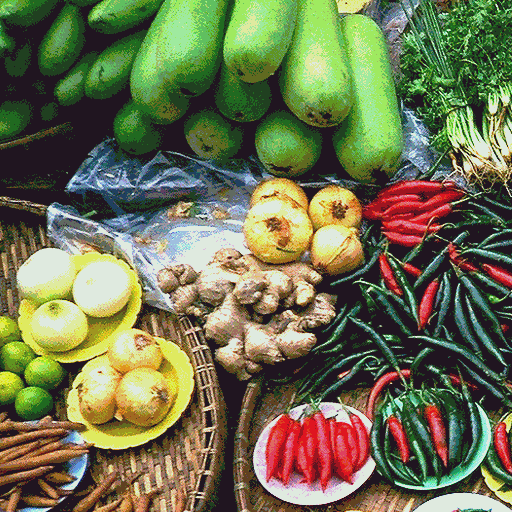
\includegraphics[width=\ww\linewidth]{../zad2/rgb4/I1_464.png }} \hfill%	
    \subfloat[Kwant. 8x8x4 \\ Liczba barw = 181 \\ PSNR = 24.3121]{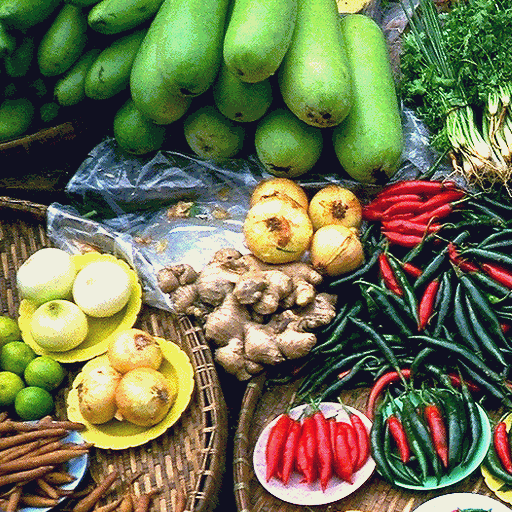
\includegraphics[width=\ww\linewidth]{../zad2/rgb4/I1_884.png }} \hfill% wypełnenie
    \caption{skwantyzowane obrazy RGB} 
    \label{fig:porownanie1} %label który można wykorzystać w tekście za pomocą polecenia \ref{fig:porownanie1}
\end{figure}

\renewcommand{\ww}{0.19} 
\begin{figure}[H]
    \captionsetup[subfloat]{justification=raggedright,singlelinecheck=false, position=bottom,labelformat=empty} %
    \subfloat[Oryginał \\ Liczba barw = 2276]{\includegraphics[width=\ww\linewidth]{../zad2/rgb5/I1_ori.png }} \hfill%	
    \subfloat[Kwant. 2x2x2 \\ Liczba barw = 8 \\ PSNR = 14.1845]{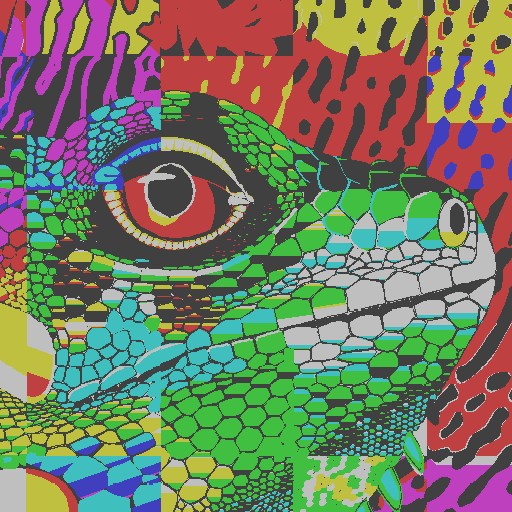
\includegraphics[width=\ww\linewidth]{../zad2/rgb5/I1_222.png }} \hfill%	
    \subfloat[Kwant. 4x4x4 \\ Liczba barw = 61 \\ PSNR = 20.2865]{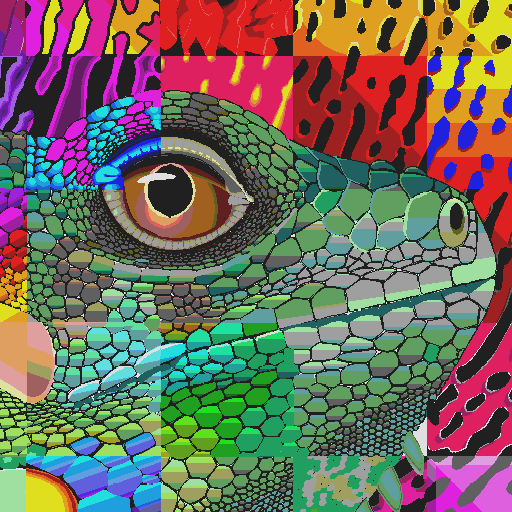
\includegraphics[width=\ww\linewidth]{../zad2/rgb5/I1_444.png }} \hfill% wypełnenie
    \subfloat[Kwant. 4x6x4 \\ Liczba barw = 86 \\ PSNR = 21.1813]{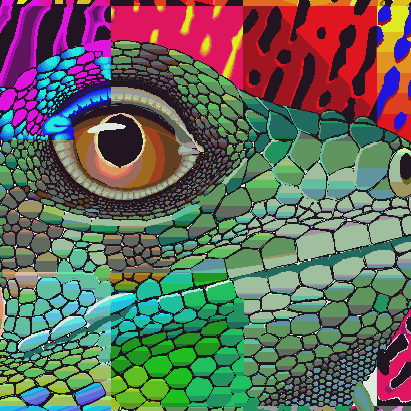
\includegraphics[width=\ww\linewidth]{../zad2/rgb5/I1_464.png }} \hfill%	
    \subfloat[Kwant. 8x8x4 \\ Liczba barw = 163 \\ PSNR = 23.3185]{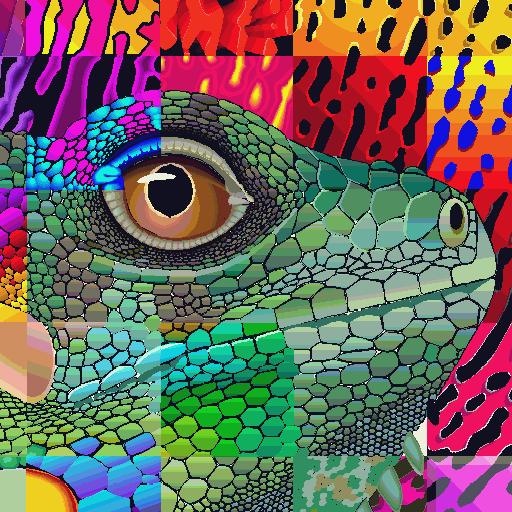
\includegraphics[width=\ww\linewidth]{../zad2/rgb5/I1_884.png }} \hfill% wypełnenie
    \caption{skwantyzowane obrazy RGB} 
    \label{fig:porownanie1} %label który można wykorzystać w tekście za pomocą polecenia \ref{fig:porownanie1}
\end{figure}


\subsection*{
    Kwantyzacja HSV
}

\renewcommand{\ww}{0.30} 
\begin{figure}[H]
    \captionsetup[subfloat]{justification=raggedright,singlelinecheck=false, position=bottom,labelformat=empty} %
    \subfloat[Oryginał \\ Liczba barw = 230651]{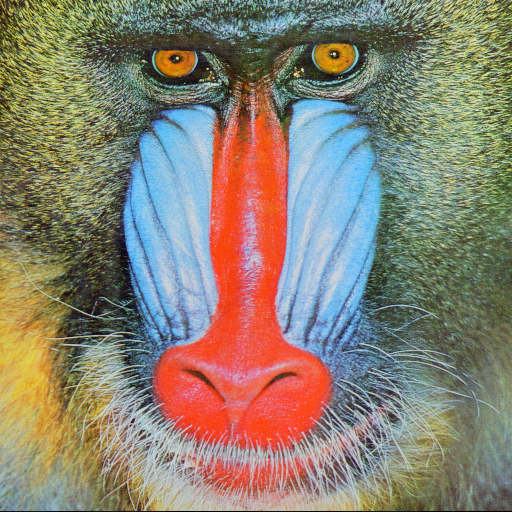
\includegraphics[width=\ww\linewidth]{../zad2/hsv1/I1_ori.png }} \hfill%	
    \subfloat[Kwant. 10x5x5+6 \\ Liczba barw = 219 \\ PSNR = 26.2205]{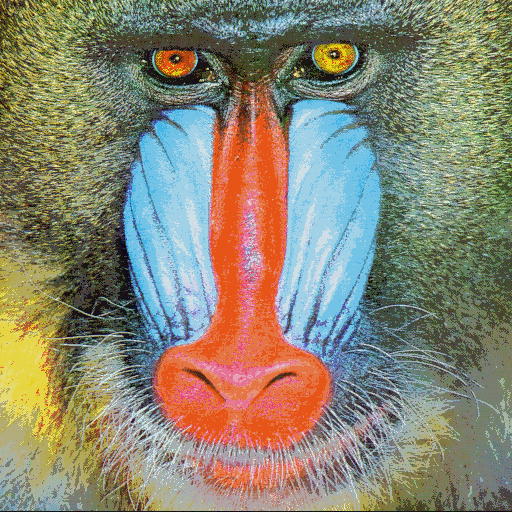
\includegraphics[width=\ww\linewidth]{../zad2/hsv1/I1_222.png }} \hfill%
    \subfloat[Kwant. 12x4x5+6 \\ Liczba barw = 214 \\ PSNR = 25.4290]{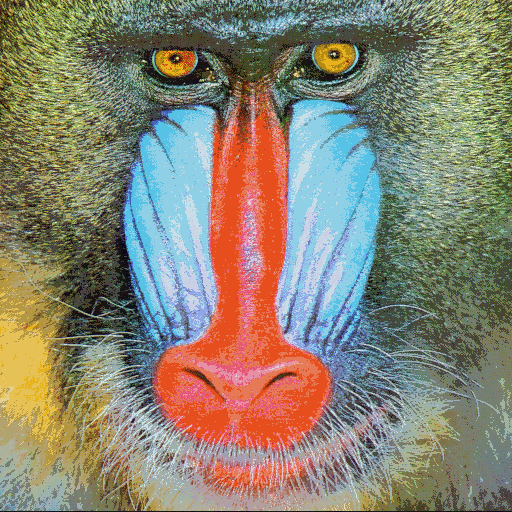
\includegraphics[width=\ww\linewidth]{../zad2/hsv1/I1_444.png }} \hfill%
    \caption{skwantyzowane obrazy HSV} 
    \label{fig:porownanie1} %label który można wykorzystać w tekście za pomocą polecenia \ref{fig:porownanie1}
\end{figure}

\begin{figure}[H]
    \captionsetup[subfloat]{justification=raggedright,singlelinecheck=false, position=bottom,labelformat=empty} %
    \subfloat[Oryginał \\ Liczba barw = 148702]{\includegraphics[width=\ww\linewidth]{../zad2/hsv2/I1_ori.png }} \hfill%	
    \subfloat[Kwant. 10x5x5+6 \\ Liczba barw = 70 \\ PSNR = 25.7836]{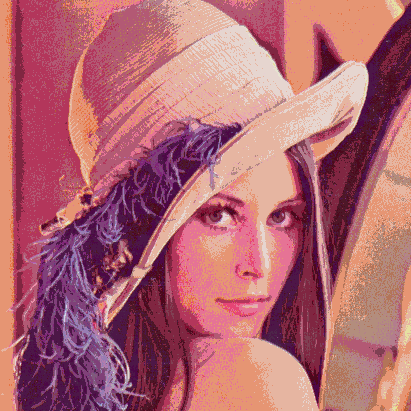
\includegraphics[width=\ww\linewidth]{../zad2/hsv2/I1_222.png }} \hfill%	
    \subfloat[Kwant. 12x4x5+6 \\ Liczba barw = 64 \\ PSNR = 25.1908]{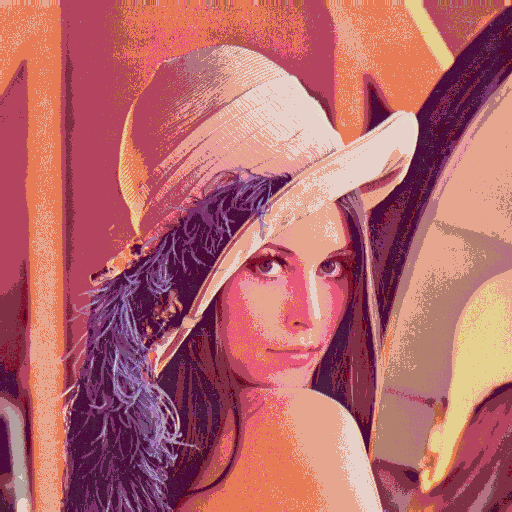
\includegraphics[width=\ww\linewidth]{../zad2/hsv2/I1_444.png }} \hfill%
    \caption{skwantyzowane obrazy HSV} 
    \label{fig:porownanie1} %label który można wykorzystać w tekście za pomocą polecenia \ref{fig:porownanie1}
\end{figure}

\begin{figure}[H]
    \captionsetup[subfloat]{justification=raggedright,singlelinecheck=false, position=bottom,labelformat=empty} %
    \subfloat[Oryginał \\ Liczba barw = 111344]{\includegraphics[width=\ww\linewidth]{../zad2/hsv3/I1_ori.png }} \hfill%	
    \subfloat[Kwant. 10x5x5+6 \\ Liczba barw = 104 \\ PSNR = 25.1388]{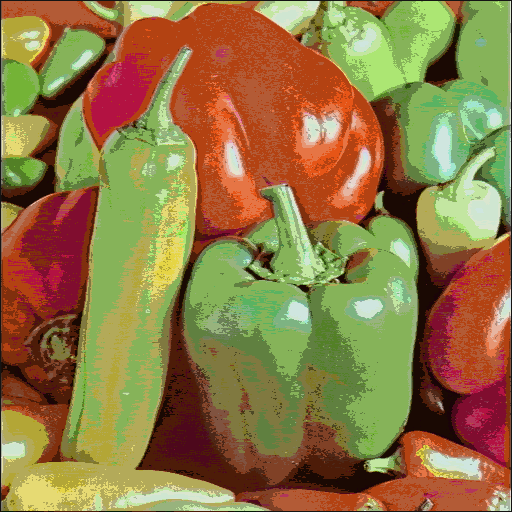
\includegraphics[width=\ww\linewidth]{../zad2/hsv3/I1_222.png }} \hfill%	
    \subfloat[Kwant. 12x4x5+6 \\ Liczba barw = 101 \\ PSNR = 24.5808]{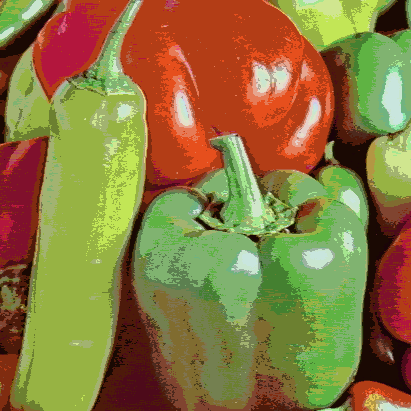
\includegraphics[width=\ww\linewidth]{../zad2/hsv3/I1_444.png }} \hfill%
    \caption{skwantyzowane obrazy HSV} 
    \label{fig:porownanie1} %label który można wykorzystać w tekście za pomocą polecenia \ref{fig:porownanie1}
\end{figure}

\begin{figure}[H]
    \captionsetup[subfloat]{justification=raggedright,singlelinecheck=false, position=bottom,labelformat=empty} %
    \subfloat[Oryginał \\ Liczba barw = 188833]{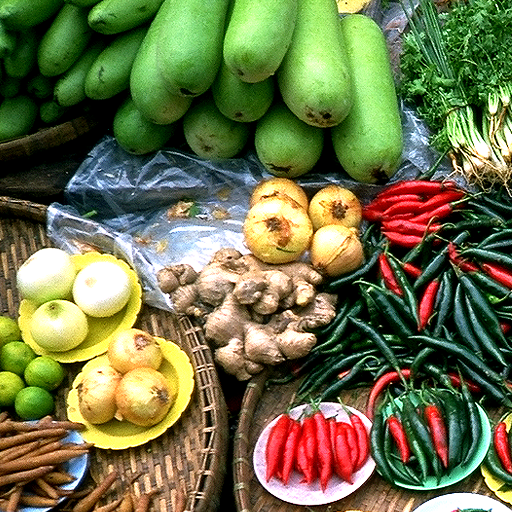
\includegraphics[width=\ww\linewidth]{../zad2/hsv4/I1_ori.png }} \hfill%	
    \subfloat[Kwant. 10x5x5+6 \\ Liczba barw = 227 \\ PSNR = 24.7579]{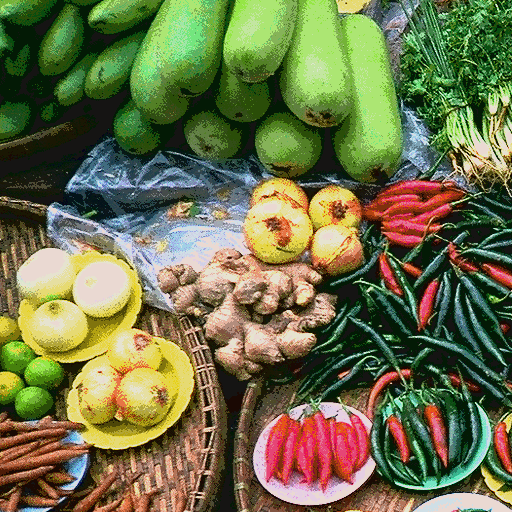
\includegraphics[width=\ww\linewidth]{../zad2/hsv4/I1_222.png }} \hfill%	
    \subfloat[Kwant. 12x4x5+6 \\ Liczba barw = 216 \\ PSNR = 23.7864]{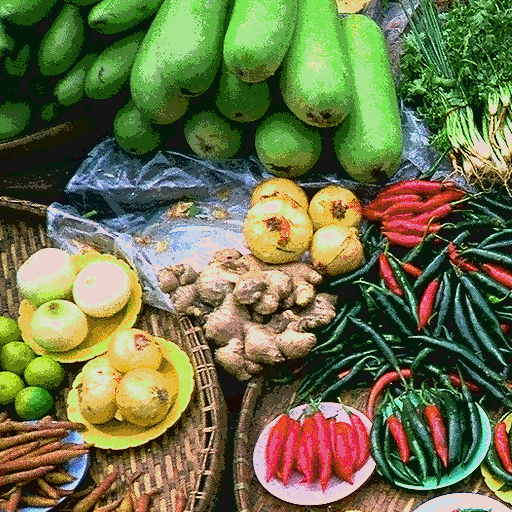
\includegraphics[width=\ww\linewidth]{../zad2/hsv4/I1_444.png }} \hfill%
    \caption{skwantyzowane obrazy HSV} 
    \label{fig:porownanie1} %label który można wykorzystać w tekście za pomocą polecenia \ref{fig:porownanie1}
\end{figure}

\begin{figure}[H]
    \captionsetup[subfloat]{justification=raggedright,singlelinecheck=false, position=bottom,labelformat=empty} %
    \subfloat[Oryginał \\ Liczba barw = 2276]{\includegraphics[width=\ww\linewidth]{../zad2/hsv5/I1_ori.png }} \hfill%	
    \subfloat[Kwant. 10x5x5+6 \\ Liczba barw = 125 \\ PSNR = 23.3403]{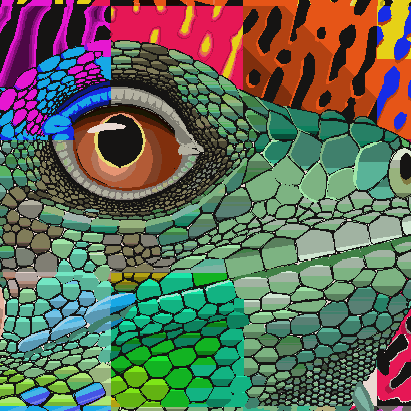
\includegraphics[width=\ww\linewidth]{../zad2/hsv5/I1_222.png }} \hfill%	
    \subfloat[Kwant. 12x4x5+6 \\ Liczba barw = 120 \\ PSNR = 22.4849]{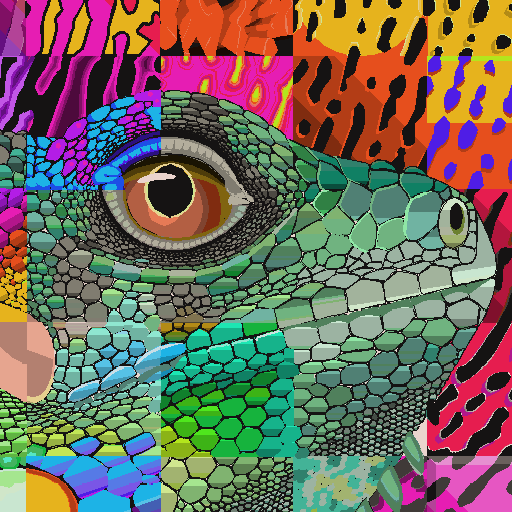
\includegraphics[width=\ww\linewidth]{../zad2/hsv5/I1_444.png }} \hfill%
    \caption{skwantyzowane obrazy HSV} 
    \label{fig:porownanie1} %label który można wykorzystać w tekście za pomocą polecenia \ref{fig:porownanie1}
\end{figure}








\newpage

\section*{Kody Programów}


\definecolor{codegreen}{rgb}{0,0.6,0}
\definecolor{codegray}{rgb}{0.5,0.5,0.5}
\definecolor{codepurple}{rgb}{0.58,0,0.82}
\definecolor{backcolour}{rgb}{0.95,0.95,0.92}

\lstdefinestyle{mystyle}{
    backgroundcolor=\color{backcolour},   
    commentstyle=\color{codegreen},
    keywordstyle=\color{magenta},
    numberstyle=\tiny\color{codegray},
    stringstyle=\color{codepurple},
    basicstyle=\ttfamily\footnotesize,
    breakatwhitespace=false,         
    breaklines=true,                 
    captionpos=b,                    
    keepspaces=true,                 
    numbers=left,                    
    numbersep=5pt,                  
    showspaces=false,                
    showstringspaces=false,
    showtabs=false,                  
    tabsize=2,
    float=H,
    extendedchars=\true, 
}


\lstset{style=mystyle}


\lstset{%
  breaklines=true
}

    
 \subsection*{count\_rgb1.m         }  \lstinputlisting[language=Octave]{../matlab/count\_rgb1.m         } \newpage      
 \subsection*{count\_rgb2.m         }  \lstinputlisting[language=Octave]{../matlab/count\_rgb2.m         } \newpage      
 \subsection*{count\_rgb3.m         }  \lstinputlisting[language=Octave]{../matlab/count\_rgb3.m         } \newpage      
 \subsection*{count\_rgb4.m         }  \lstinputlisting[language=Octave]{../matlab/count\_rgb4.m         } \newpage      
 \subsection*{count\_test.m         }  \lstinputlisting[language=Octave]{../matlab/count\_test.m         } \newpage      
 \subsection*{image\_quantization.m }  \lstinputlisting[language=Octave]{../matlab/image\_quantization.m } \newpage              
 \subsection*{quantization\_test.m  }  \lstinputlisting[language=Octave]{../matlab/quantization\_test.m  } \newpage             
 \subsection*{zad1.m                }  \lstinputlisting[language=Octave]{../matlab/zad1.m               } \newpage
 \subsection*{zad2.m                }  \lstinputlisting[language=Octave]{../matlab/zad2.m }




\end{document}